\begin{priprava}{9., 10., 11., 12., 13}{}{Operacije z množicami}{Osnove logike in teorije množic}{frontalna}{drsnice, projekcija, tabla}


    \section{Operacije z množicami}

    \subsection{Komplement množice}
    
                \textbf{Komplement} množice $\mathcal{A}$ (glede na izbrani univerzum $\mathcal{U}$) je množica 
                vseh elementov, ki so v množici $\mathcal{U}$ in niso v množici $\mathcal{A}$.

                Oznaka: $\mathbf{\mathcal{A}^\complement}$ / $\mathbf{\mathcal{A}'}$.      
                $$ \mathcal{A}^\complement=\left\{ x; x\in\mathcal{U}\land x\notin\mathcal{A}\right\} $$           
            

            \begin{figure}[H]
                \centering
                \begin{tikzpicture}                     
                    \draw[fill=red!70,fill opacity=0.5]  (-3,-1.5)  rectangle (3,1.5);
                
                    % \draw[fill=blue!70,fill opacity=0.5] (0,0) ellipse (2.5cm and 1.2cm);
                    \draw[fill=white,fill opacity=1] (-0.6,-0.3) ellipse (1.5cm and 0.8cm);
                    
                    \node at (-1,-0.3) {$\mathcal{A}$};
                    \node at (1.7,0) {$\mathcal{A}^\complement$};
                    % \node at (0,1.1) {$\mathcal{A}^\complement$};
                    \node at (-2.7,-1.2) {$\mathcal{U}$};
                    
                \end{tikzpicture}
            \end{figure}

        $$\left( \mathcal{A}^\complement\right)^\complement=\mathcal{A} $$
        
        \begin{naloga}
            Naj bo univerzalna množica $\mathcal{U}=\{x; x\in\mathbb{N} \land x\leq 20\}$. 
            Zapišite komplementarno množico danih množic. Kakšna je njena mmoč?
            \begin{itemize}
                \item $\mathcal{A}=\{x; x=3k \land k\in\mathbb{N}\}$
                \item $\mathcal{B}=\{x; x\in\mathbb{N} \land x\mid 20\}$
                \item $\mathcal{C}=\{x; x=2k \lor x=3k \land k\in\mathbb{N}\}$
            \end{itemize}
        \end{naloga}



    \subsection{Unija množic}
                \textbf{Unija} množic $\mathcal{A}$ in $\mathcal{B}$ je množica vseh elementov, ki pripadajo 
                množici $\mathcal{A}$ ali množici $\mathcal{B}$.

                Oznaka: $\mathbf{\mathcal{A}\cup\mathcal{B}}$.
                $$ \mathcal{A}\cup\mathcal{B}=\left\{x; x\in\mathcal{A}\lor x\in\mathcal{B}\right\} $$



        \begin{figure}[H]
            \centering
            \begin{subfigure}[b]{0.4\textwidth}
                \centering
                            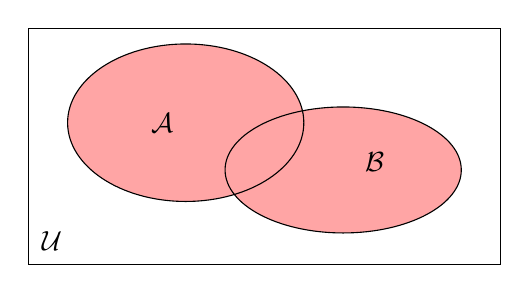
\begin{tikzpicture}                     
                \draw  (-3,-1.5)  rectangle (3,1.5);
            
                \draw[fill=red!70,fill opacity=0.5] (-1,0.3) ellipse (1.5cm and 1cm)
                                                    (1,-0.3) ellipse (1.5cm and 0.8cm);
                
                \node at (-1.3,0.3) {$\mathcal{A}$};
                \node at (1.4,-0.2) {$\mathcal{B}$};
                % \node at (0,1.1) {$\mathcal{A}\cup\mathcal{B}$};
                \node at (-2.7,-1.2) {$\mathcal{U}$};
                
            \end{tikzpicture}

            \end{subfigure}
            \begin{subfigure}[b]{0.4\textwidth}
                \centering
                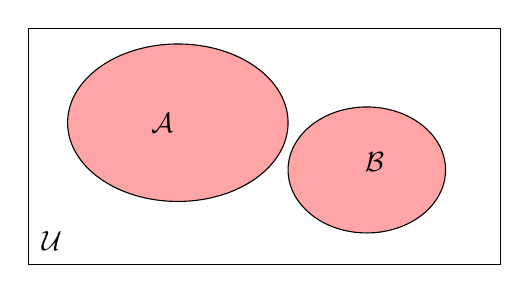
\begin{tikzpicture}                     
                \draw  (-3,-1.5)  rectangle (3,1.5);
            
                \draw[fill=red!70,fill opacity=0.5] (-1.1,0.3) ellipse (1.4cm and 1cm)
                                                    (1.3,-0.3) ellipse (1cm and 0.8cm);
                
                \node at (-1.3,0.3) {$\mathcal{A}$};
                \node at (1.4,-0.2) {$\mathcal{B}$};
                % \node at (0,1.1) {$\mathcal{A}\cup\mathcal{B}$};
                \node at (-2.7,-1.2) {$\mathcal{U}$};
                
            \end{tikzpicture}
        \end{subfigure}
    \end{figure}


                $$ \mathcal{A}\cup\mathcal{A}^\complement=\mathcal{U}$$
                $$ \mathcal{A}\cup\emptyset=\mathcal{A}$$
                $$ \mathcal{A}\cup\mathcal{U}=\mathcal{U}$$
            


                \begin{naloga}
                    Dani sta množici $\mathcal{A}$ in $\mathcal{B}$. Zapišite množico $\mathcal{A}\cup\mathcal{B}$.
                    Določite še njeno moč.
                    \begin{itemize}
                        \item $\mathcal{A}=\{1,2,3,4,5\}$ in $\mathcal{B}=\{3,4,5,6,7\}$
                        \item $\mathcal{A}=\{4,8,12,16,20\}$ in $\mathcal{B}=\{3,6,9,12,15,18\}$
                        \item $\mathcal{A}=\{x; x\in\mathbb{N} \land x\mid 18\}$ in $\mathcal{B}=\{x; x\in\mathbb{N} \land x\mid 21\}$
                        \item $\mathcal{A}=\{5,10,15,20,\dots\}$ in $\mathcal{B}=\{10, 20, 30, 40, 50, \dots\}$
                        \item $\mathcal{A}=\{x; x=6k \land k\in\mathbb{N} \land k\leq 4\}$ in $\mathcal{B}=\{x; x\in\mathbb{N} \land x\mid 12\}$
                    \end{itemize}
                \end{naloga}
        




\subsection{Presek množic}
            \textbf{Presek} množic $\mathcal{A}$ in $\mathcal{B}$ je množica vseh elementov, ki hkrati 
            pripadajo množici $\mathcal{A}$ in množici $\mathcal{B}$.

            Oznaka: $\mathbf{\mathcal{A}\cap\mathcal{B}}$.
            $$ \mathcal{A}\cap\mathcal{B}=\left\{x; x\in\mathcal{A}\land x\in\mathcal{B}\right\} $$
        

            \begin{figure}[H]
                \centering
                \begin{subfigure}[b]{0.4\textwidth}
                    \centering
                    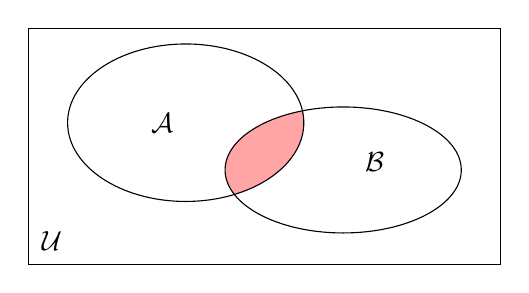
\begin{tikzpicture}                     
                \draw  (-3,-1.5)  rectangle (3,1.5);

                \begin{scope}
                    \clip (-1,0.3) ellipse (1.5cm and 1cm);
                    \fill[fill=red!70,fill opacity=0.5] (1,-0.3) ellipse (1.5cm and 0.8cm);
                \end{scope}
                \draw (-1,0.3) ellipse (1.5cm and 1cm);
                \draw (1,-0.3) ellipse (1.5cm and 0.8cm);
                
                \node at (-1.3,0.3) {$\mathcal{A}$};
                \node at (1.4,-0.2) {$\mathcal{B}$};
                % \node at (0,1.1) {$\mathcal{A}\cap\mathcal{B}$};
                \node at (-2.7,-1.2) {$\mathcal{U}$};
                
            \end{tikzpicture}
        \end{subfigure}
        \begin{subfigure}[b]{0.4\textwidth}
            \centering
                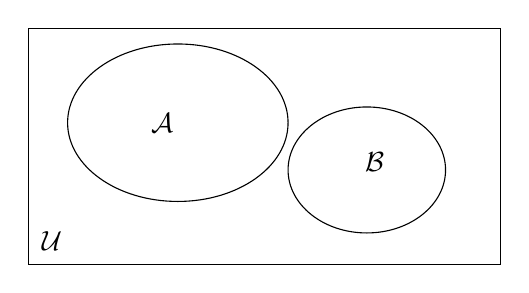
\begin{tikzpicture}                     
                \draw  (-3,-1.5)  rectangle (3,1.5);
            
                \draw (-1.1,0.3) ellipse (1.4cm and 1cm)
                    (1.3,-0.3) ellipse (1cm and 0.8cm);
                
                \node at (-1.3,0.3) {$\mathcal{A}$};
                \node at (1.4,-0.2) {$\mathcal{B}$};
                % \node at (0,1.1) {$\mathcal{A}\cap\mathcal{B}$};
                \node at (-2.7,-1.2) {$\mathcal{U}$};
                
            \end{tikzpicture}
        \end{subfigure}
    \end{figure}


            $$ \mathcal{A}\cap\mathcal{A}^\complement=\emptyset$$
            $$ \mathcal{A}\cap\emptyset=\emptyset$$
            $$ \mathcal{A}\cap\mathcal{U}=\mathcal{A}$$



            \begin{naloga}
                Dani sta množici $\mathcal{A}$ in $\mathcal{B}$. Zapišite množico $\mathcal{A}\cap\mathcal{B}$.
                Določite še njeno moč.
                \begin{itemize}
                    \item $\mathcal{A}=\{1,2,3,4,5\}$ in $\mathcal{B}=\{3,4,5,6,7\}$
                    \item $\mathcal{A}=\{4,8,12,16,20\}$ in $\mathcal{B}=\{3,6,9,12,15,18\}$
                    \item $\mathcal{A}=\{x; x\in\mathbb{N} \land x\mid 18\}$ in $\mathcal{B}=\{x; x\in\mathbb{N} \land x\mid 21\}$
                    \item $\mathcal{A}=\{5,10,15,20,\dots\}$ in $\mathcal{B}=\{10, 20, 30, 40, 50, \dots\}$
                    \item $\mathcal{A}=\{x; x=6k \land k\in\mathbb{N} \land k\leq 4\}$ in $\mathcal{B}=\{x; x\in\mathbb{N} \land x\mid 12\}$
                \end{itemize}
            \end{naloga}
    
~

    Za množici $\mathcal{A}$ in $\mathcal{B}$ velja:
    $$m(\mathcal{A}\cup\mathcal{B})=m(\mathcal{A})+m(\mathcal{B})-m(\mathcal{A}\cap\mathcal{B}) $$



    Množici, katerih presek je prazna množica, sta \textbf{disjunktni} množici.
    $$\mathcal{A}\cap\mathcal{B}=\emptyset\Rightarrow m(\mathcal{A}\cap\mathcal{B})=0 $$ 
    $$\mathcal{A}\cap\mathcal{B}=\emptyset\Rightarrow m(\mathcal{A}\cup\mathcal{B})=m(\mathcal{A})+m(\mathcal{B}) $$


\subsection{Lastnosti operacij unije in preseka}
        \subsubsection{Komutativnost unije in preseka}
            $$ \mathcal{A}\cup\mathcal{B}=\mathcal{B}\cup\mathcal{A} $$
            $$ \mathcal{A}\cap\mathcal{B}=\mathcal{B}\cap\mathcal{A} $$
        

            \subsubsection{Asociativnost unije in preseka}
            $$ \left(\mathcal{A}\cup\mathcal{B}\right)\cup\mathcal{C}=\mathcal{A}\cup\left(\mathcal{B}\cup\mathcal{C}\right) $$
            $$ \left(\mathcal{A}\cap\mathcal{B}\right)\cap\mathcal{C}=\mathcal{A}\cap\left(\mathcal{B}\cap\mathcal{C}\right) $$


            \subsubsection{Distributivnostna zakona za unijo in presek}
    $$ \left(\mathcal{A}\cup\mathcal{B}\right)\cap\mathcal{C}=\left(\mathcal{A}\cap\mathcal{C}\right)\cup\left(\mathcal{B}\cap\mathcal{C}\right) $$
    $$ \left(\mathcal{A}\cap\mathcal{B}\right)\cup\mathcal{C}=\left(\mathcal{A}\cup\mathcal{C}\right)\cap\left(\mathcal{B}\cup\mathcal{C}\right) $$


    \subsubsection{De Morganova zakona}
    Komplement preseka dveh množic je enak uniji komplementov obeh množic:
    $$\left(\mathcal{A}\cap\mathcal{B}\right)^\complement=\mathcal{A}^\complement\cup\mathcal{B}^\complement. $$
    Komplement unije dveh množic je enak preseku komplementov obeh množic:
    $$\left(\mathcal{A}\cup\mathcal{B}\right)^\complement=\mathcal{A}^\complement\cap\mathcal{B}^\complement. $$







        \subsection{Razlika množic}
            \textbf{Razlika} množic $\mathcal{A}$ in $\mathcal{B}$ je množica tistih elementov, ki  
            pripadajo množici $\mathcal{A}$ in hkrati ne pripadajo množici $\mathcal{B}$.

            Oznaka: $\mathbf{\mathcal{A}\setminus\mathcal{B}}$ / $\mathbf{\mathcal{A}-\mathcal{B}}$.
            $$ \mathcal{A}\setminus\mathcal{B}=\left\{x; x\in\mathcal{A}\land x\notin\mathcal{B}\right\} $$
        

        
        


            \begin{figure}[H]
                \centering
                \begin{subfigure}[b]{0.4\textwidth}
                    \centering
            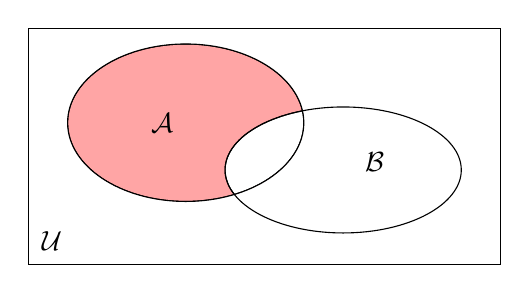
\begin{tikzpicture}                     
                \draw  (-3,-1.5)  rectangle (3,1.5);

                \begin{scope}
                    \clip (-1,0.3) ellipse (1.5cm and 1cm);
                    \draw[fill=red!70,fill opacity=0.5, even odd rule] (-1,0.3) ellipse (1.5cm and 1cm)
                                (1,-0.3) ellipse (1.5cm and 0.8cm);
                \end{scope}

                \draw (-1,0.3) ellipse (1.5cm and 1cm);
                \draw (1,-0.3) ellipse (1.5cm and 0.8cm);
                
                \node at (-1.3,0.3) {$\mathcal{A}$};
                \node at (1.4,-0.2) {$\mathcal{B}$};
                % \node at (0,1.1) {$\mathcal{A}\setminus\mathcal{B}$};
                \node at (-2.7,-1.2) {$\mathcal{U}$};
                
            \end{tikzpicture}
        \end{subfigure}
        \begin{subfigure}[b]{0.4\textwidth}
            \centering
        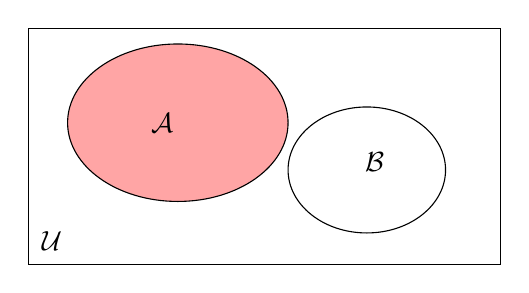
\begin{tikzpicture}                     
                \draw  (-3,-1.5)  rectangle (3,1.5);
            
                \draw[fill=red!70,fill opacity=0.5] (-1.1,0.3) ellipse (1.4cm and 1cm);
                \draw                               (1.3,-0.3) ellipse (1cm and 0.8cm);
                
                \node at (-1.3,0.3) {$\mathcal{A}$};
                \node at (1.4,-0.2) {$\mathcal{B}$};
                % \node at (0,1.1) {$\mathcal{A}\setminus\mathcal{B}$};
                \node at (-2.7,-1.2) {$\mathcal{U}$};
                
            \end{tikzpicture}
        \end{subfigure}
    \end{figure}



            $$ \mathcal{A}\setminus\mathcal{B}=\mathcal{A}\cap\mathcal{B}^\complement$$
            $$ \mathcal{A}\setminus\mathcal{B}\neq\mathcal{B}\setminus\mathcal{A}$$
            $$ \mathcal{A}\setminus\mathcal{A}=\emptyset$$


            \begin{naloga}
                Dani sta množici $\mathcal{A}$ in $\mathcal{B}$. Zapišite njuno razliko $\mathcal{A}\setminus\mathcal{B}$.
                \begin{itemize}
                    \item $\mathcal{A}=\{2,4,6,8,10,12,14,16,18,20\}$ in $\mathcal{B}=\{x; x\in\mathbb{N} \land x>10\}$
                    \item $\mathcal{A}=\{x; x=3k \land k\in\mathbb{N} \land k<7\}$ in $\mathcal{B}=\{x; x=6k \land k\in\mathbb{N}\}$
                    \item $\mathcal{A}=\{x; x=6k \land k\in\mathbb{N} \land k<4\}$ in $\mathcal{B}=\{x; x=3k \land k\in\mathbb{N}\}$
                \end{itemize}
            \end{naloga}



        \subsection{Kartezični produkt množic}
            \textbf{Kartezični produkt} (nepraznih) množic $\mathcal{A}$ in $\mathcal{B}$ je množica 
            urejenih parov $(x,y)$, pri čemer je $x\in\mathcal{A}$ in $y\in\mathcal{B}$.

            Oznaka: $\mathbf{\mathcal{A}\times\mathcal{B}}$.
            $$ \mathcal{A}\times\mathcal{B}=\left\{(x,y); x\in\mathcal{A}\land y\in\mathcal{B}\right\} $$
        

        
            $$x\neq y \Rightarrow (x,y)\neq(y,x)$$
            $$\mathcal{A}\neq\mathcal{B}\Rightarrow \mathcal{A}\times\mathcal{B}\neq\mathcal{B}\times\mathcal{A}$$
        
    
            $$m(\mathcal{A}\times\mathcal{B})=m(\mathcal{A})\cdot m(\mathcal{B}) $$
        \newline

              Kartezični produkt $\mathcal{A}\times\mathcal{B}$ za množici $ \mathcal{A}=\left\{a,b,c,d,e,f\right\}$ in
              $ \mathcal{B}=\left\{1,2,3,4\right\}$:

            \begin{figure}[H]  
                \centering                   
                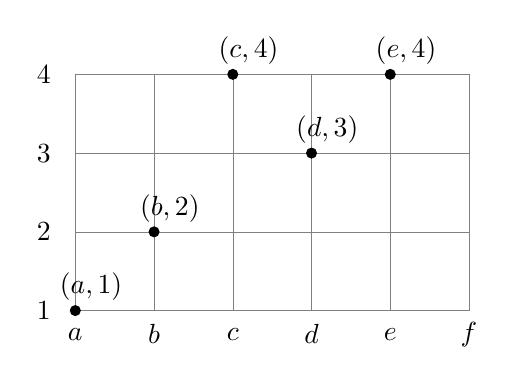
\begin{tikzpicture}
                \draw[help lines] (0,0) grid (5,3);
              
                \fill (1,1) circle (2pt);
                \fill (3,2) circle (2pt);
                \fill (2,3) circle (2pt);
                \fill (4,3) circle (2pt);
                \fill (0,0) circle (2pt);

                \node at (0,-0.3) {$a$};
                \node at (1,-0.3) {$b$};
                \node at (2,-0.3) {$c$};
                \node at (3,-0.3) {$d$};
                \node at (4,-0.3) {$e$};
                \node at (5,-0.3) {$f$};
                \node at (-0.4,0) {$1$};
                \node at (-0.4,1) {$2$};
                \node at (-0.4,2) {$3$};
                \node at (-0.4,3) {$4$};

                \node at (0.2,0.3) {$(a,1)$};
                \node at (1.2,1.3) {$(b,2)$};
                \node at (2.2,3.3) {$(c,4)$};
                \node at (3.2,2.3) {$(d,3)$};
                \node at (4.2,3.3) {$(e,4)$};

              \end{tikzpicture}
            \end{figure}

            \begin{naloga}
                Dani sta množici $\mathcal{A}$ in $\mathcal{B}$. Zapišite njun kartezični produkt $\mathcal{A}\times\mathcal{B}$.
                Narišite diagram, ki predstavlja to množico.
                \begin{itemize}
                    \item $\mathcal{A}=\{2,4,6,8,10,12\}$ in $\mathcal{B}=\{x; x\in\mathbb{N} \land x<8\}$
                    \item $\mathcal{A}=\{x; x=3k \land k\in\mathbb{N} \land k < 7\}$ in $\mathcal{B}=\{x; x=6k \land k\in\mathbb{N}\land (5\leq k<9)\}$
                    \item $\mathcal{A}=\{x; x=6k \land k\in\mathbb{N} \land k<4\}$ in $\mathcal{B}=\{x; x=3k \land k\in\mathbb{N}\land (3<k<11)\}$
                \end{itemize}
            \end{naloga}
    
    
              


\end{priprava}